\documentclass[../main.tex]{subfiles}
\graphicspath{{\subfix{../img/}}}
\begin{document}

\newpage
\section{Aufgabenstellung}
Im Projektmodul \acrfull{pren1} an der Hochschule Luzern im Herbstsemester 2024 steht die Entwicklung eines autonomen Fahrzeugs im Mittelpunkt. Dieses Fahrzeug soll sich auf einem vorgegebenen Wege-Netzwerk eigenständig bewegen und dabei den optimalen Weg zum Ziel finden. Das gesamte System muss ohne externe Eingriffe arbeiten und selbstständig Entscheidungen treffen. 

Das Wege-Netzwerk besteht aus 8 fixierten Wegpunkten, die durch Linien aus Klebeband verbunden sind. Eine zentrale Herausforderung besteht darin, dass das Fahrzeug während der Fahrt gesperrte Wegpunkte vermeiden und Hindernisse erkennen und korrekt behandeln soll. Zusätzlich gibt es bestimmte Abschnitte des Wegenetzes, die von den Dozenten entfernt werden können, was das Fahrzeug ebenfalls berücksichtigen muss. 

Das Projekt wird in zwei Phasen unterteilt: In \acrshort{pren1}, das im Herbstsemester stattfindet, steht die Konzeptentwicklung im Vordergrund. Die Studierenden erarbeiten ein Gesamtkonzept, das alle relevanten Teilfunktionen des Fahrzeugs berücksichtigt. Parallel dazu wird ein Simulator entwickelt, mit dem die geplanten Fahrwege und Reaktionen auf Hindernisse und Sperrungen getestet werden können. Dieser Simulator soll den Entwicklungsprozess unterstützen und dokumentiert werden. 

Im darauffolgenden Frühlingssemester, \acrshort{pren2}, wird auf Basis des erarbeiteten Konzepts ein funktionaler Prototyp gebaut. Das fertige Fahrzeug tritt schliesslich in einem Wettbewerb gegen die Fahrzeuge anderer Teams an, wobei es auf Zuverlässigkeit und Effizienz geprüft wird. Hierbei wird bewertet, ob das Fahrzeug regelkonform fährt, Hindernisse richtig handhabt und das Ziel möglichst schnell erreicht. 

Ein besonderes Augenmerk liegt zudem auf der Nachhaltigkeit des Projekts. Die Studierenden sollen bereits, während der Konzeptphase Aspekte wie Materialwahl, Energieverbrauch und Recycling-Möglichkeiten berücksichtigen. Diese Nachhaltigkeitsüberlegungen sind auch Teil der abschliessenden Bewertung. Der Projektverlauf wird in Form einer Dokumentation festgehalten, die später als Beispiel für zukünftige Projektarbeiten dienen soll.

Die originale Aufgabenstellung befindet sich im Anhang \ref{aufgabenstellung}.

\newpage
\subsection{Skizze Aufgabenstellung}
Die Skizze soll die Aufgabenstellung visuell darstellen und dadurch eine  Übersicht über die einzelnen Anforderungen und Funktionen des Fahrzeuges schaffen.
    \begin{figure}[H]
        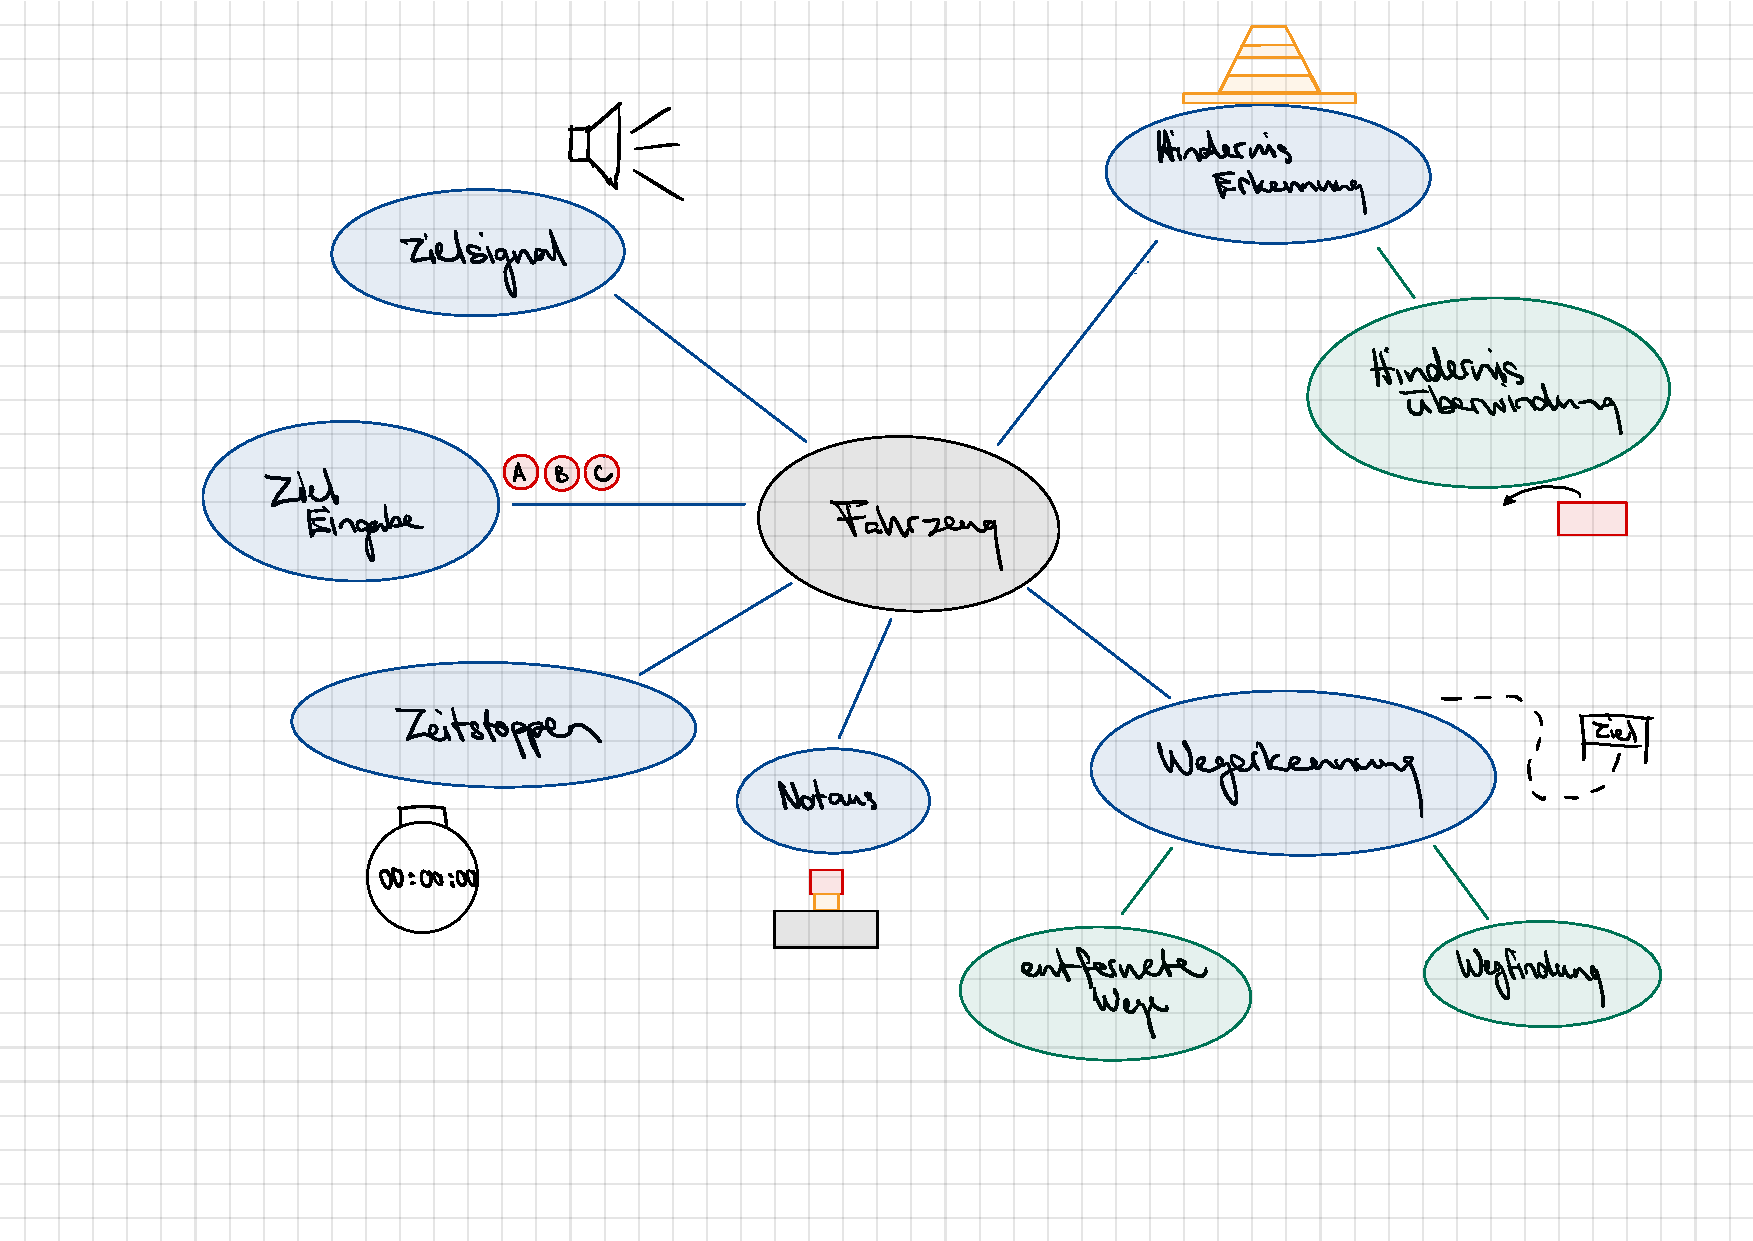
\includegraphics[width=\textwidth]{assets/Skizze_Aufgabenstellung.pdf}
        \caption{Skizze der Aufgabestellung}
        \label{img:Skizze_Aufgabenstellung}
    \end{figure} 
 
\end{document}